% --------------------------------------
% Document Class
% --------------------------------------
\documentclass[a4paper,11pt]{article}
% --------------------------------------



% --------------------------------------
% Use Package
% --------------------------------------


\usepackage[francais]{babel}
%\usepackage{ucs}
\usepackage[utf8]{inputenc}
\usepackage[T1]{fontenc}

\usepackage{makeidx}
\usepackage{color}
\usepackage{graphicx}
\usepackage{float}
\usepackage[hidelinks]{hyperref} 
\usepackage{geometry}
%\usepackage{lastpage}
%\usepackage{marginnote}
\usepackage{fancyhdr}
%\usepackage{titlesec}
%\usepackage{framed}
\usepackage{amsmath}
\usepackage{empheq}
\usepackage{array}
\usepackage{multicol}
\usepackage{csquotes}
%\usepackage{adjustbox}

% insert code
\usepackage{listings}

% define our color
\usepackage{xcolor}

% code color
\definecolor{ligthyellow}{RGB}{250,247,220}
\definecolor{darkblue}{RGB}{5,10,85}
\definecolor{ligthblue}{RGB}{1,147,128}
\definecolor{darkgreen}{RGB}{8,120,51}
\definecolor{darkred}{RGB}{160,0,0}

% other color
\definecolor{ivi}{RGB}{141,107,185}


\lstset{
    language=java,
    captionpos=b,
    extendedchars=true,
    frame=lines,
    numbers=left,
    numberstyle=\tiny,
    numbersep=5pt,
    keepspaces=true,
    breaklines=true,
    showspaces=false,
    showstringspaces=false,
    breakatwhitespace=false,
    stepnumber=1,
    showtabs=false,
    tabsize=3,
    basicstyle=\small\ttfamily,
    backgroundcolor=\color{ligthyellow},
    keywordstyle=\color{ligthblue},
    morekeywords={include, printf, uchar},
    identifierstyle=\color{darkblue},
    commentstyle=\color{darkgreen},
    stringstyle=\color{darkred},
}


% --------------------------------------



% --------------------------------------
% Page setting
% --------------------------------------
%\pagestyle{empty}
\setlength{\headheight}{15pt}

\setcounter{secnumdepth}{3}
\setcounter{tocdepth}{2}

\makeatletter
\@addtoreset{chapter}{part}
\makeatother 

\hypersetup{         % parametrage des hyperliens
  colorlinks=true,      % colorise les liens
  breaklinks=true,      % permet les retours à la ligne pour les liens trop longs
  urlcolor= blue,       % couleur des hyperliens
  linkcolor= black,     % couleur des liens internes aux documents (index, figures, tableaux, equations,...)
  citecolor= green      % couleur des liens vers les references bibliographiques
}

% --------------------------------------

% --------------------------------------
% Information
% --------------------------------------
\title{Compte-rendu TP12 TI : Compression d'image}
\author{Elliot VANEGUE et Gaëtan DEFLANDRE}
% --------------------------------------

\definecolor{myColor}{rgb}{0.5, 0.1, 0.75}

% --------------------------------------
% Begin content
% --------------------------------------
\begin{document}

% Set language to english
  \selectlanguage{francais}

  % Start the page counting
  \pagenumbering{arabic}

  \maketitle
  
  \mbox{}
  \newpage
  \clearpage
  
  \section{Introduction}
  Le transfert et le stockage d'image sont de plus en plus fréquents et nécessitent parfois de limiter la taille
  des fichiers. Pour cela il existe des algorithmes de compression d'image, dans certains cas il faut trouver 
  un compromis entre le taux de compression et la qualité de l'image. Lors de ce TP, nous allons voir comment 
  est réalisée la compression JPEG utilisée dans le format JPG.
  
  \section{Transformée en cosinus discrète}
  La transformée en cosinus discrète est une transformation ressemblant à la transformée de Fourier sauf
  que sa projection crée des coefficients réels. Le calcul de cette transformée nous est fourni pour une dimension.
  On peut voir que la fonction prend en paramètre un tableau à une dimension représentant le signal que nous allons traiter.
  La sortie de la fonction est un tableau de même taille correspondant au signal transformé par la transformée
  en cosinus discrète. Pour la fonction inverse, l'entrée et la sortie de la fonction sont échangées.\\
  
  Dans un premier temps la fonction calcule les deux facteurs de normalisation $\sqrt{\frac{2}{M}}$ où M est
  la taille du signal passé en paramètre, et $c(u)$ qui vaut 1 si $u$ est différent de 0 et $\frac{1}{\sqrt{2}}$ sinon.
  Le paramètre \enquote{u} est la position de la donnée calculée. 
  Et enfin, pour calculer une donnée la fonction
  fait la somme de toutes les autres multiplier par le cosinus de $\pi * \frac{(2m+1)*u}{2M}$ où \enquote{m}
  est la position du pixel courant.\\
  
  La propriété de séparabilité de la transformé en cosinus nous permet d'appliquer le calcul d'une dimension
  pour les deux dimensions que nous allons traiter. Ainsi, nous ne faisons que réutiliser ce calcul pour les lignes, puis pour les
  colonnes. Nous obtenons ainsi la matrice suivante :
  
  \begin{figure}[H]
    \center
   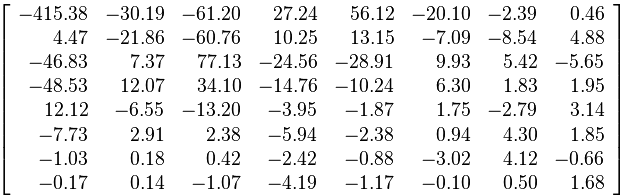
\includegraphics[width=10cm]{matrice_cosinus.png}
  \end{figure}

  Nous pouvons voir que cette matrice ne permet pas encore de diminuer la quantité de données d'une image, car il n'y a pas de valeur 
  nulle dans la matrice. Cependant, nous remarquons que les normes des valeurs en haut à gauche de la matrice sont bien plus grandes 
  que celles en bas à droite. Nous allons voir comment utiliser ce calcul pour réduire la quantité de données d'une image de beaucoup 
  plus grande taille.
  
  %orthographe ok jusqu'ici
  \section{Utilisation de la DCT pour la compression JPEG}
  Le coût en calcul pour la transformé en cosinus discrète étant assez important, nous allons travailler sur des ROI\footnote{Region Of Interest}
  que nous allons placer dans l'image. Nous allons donc découper l'image en 8x8, puis appliquer la transformé sur chacune de ces parties.\\
  
  Nous allons maintenant passer à la phase de quantification. Comme nous l'avons vu dans la partie précédente, nous avons, suite à
  l'application de la transformé en cosinus discrète, une matrice possédant des valeurs plus importantes dans son coin supérieur
  gauche. La compression JPEG étant destructrice nous allons chercher à minimiser l'impact de la compression sur l'image.
  Pour cela nous gardons les normes des valeurs les plus hautes qui correspondent aux basses fréquences. Cela va atténuer
  les informations de contour de l'image, tout en gardant les contours les plus importants. Donc nous diminuons les
  détails de l'image.\\
  
  Nous allons donc effectuer une division bit à bit entre la matrice que nous avons obtenue dans la partie précédente 
  et la matrice suivante : 
  \begin{figure}[H]
    \center
   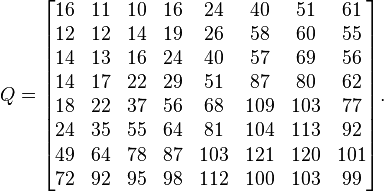
\includegraphics[width=10cm]{quantification.png}
  \end{figure}
  
  \section{Qualité et performance de la compression JPEG}
  Afin de déterminer les données qui ont été supprimées lors de la compression, nous effectuons une décompression de l'image.
  Pour cela, nous effectuons les opérations inverses de ce qui a été fait précédemment. Nous obtenons ainsi l'image suivante :
  \begin{figure}[H]
    \center
   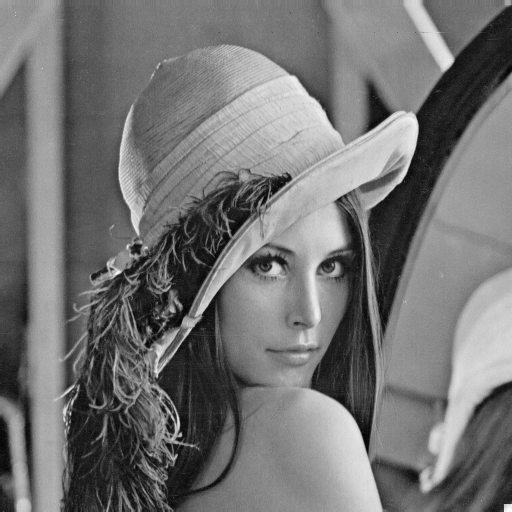
\includegraphics[width=5cm]{../result_lena.png}
   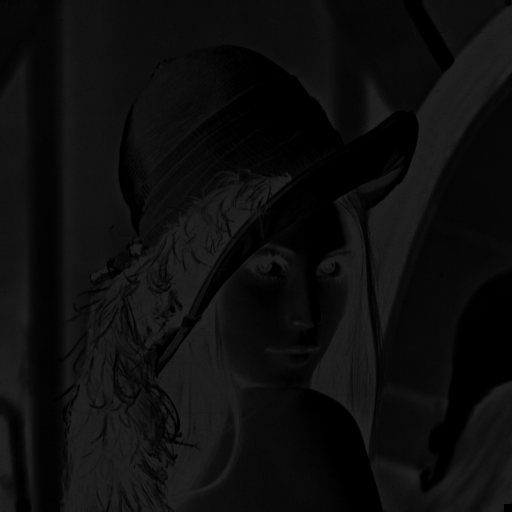
\includegraphics[width=5cm]{../diff_lena.png}
   \caption{Résultat de la décompression de l'image de Lena et différence entre l'original et la décompression}
  \end{figure}
  
  Comme nous l'avons précisé précédemment on voit que les informations qui ont été enlevées lors de la compression sont 
  des détails dans l'image.\\
  
  Il est possible de régler la qualité de la compression de l'image grâce à un facteur appliqué à la matrice de quantification.
  Ce coefficients varie entre 1 et 100, plus la valeur est importante et moins il y a de compression et donc la qualité est bonne.\\
  
  \begin{tabular}{|c|c|c|}
   \hline
   Valeur de q & Image décompressée & Différence entre originale et décompressée \\
   \hline
   q = 5  & 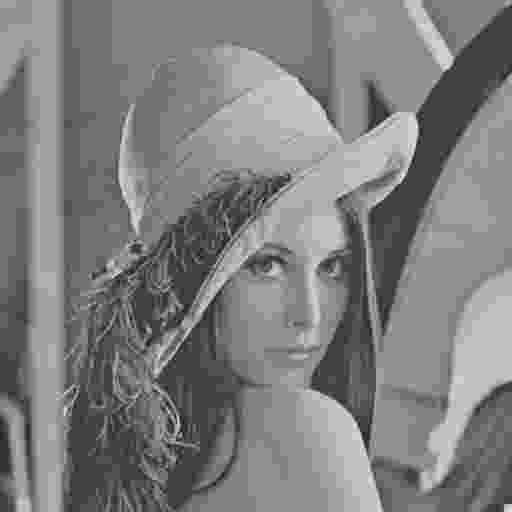
\includegraphics[width=5cm]{lena_q5.png} & 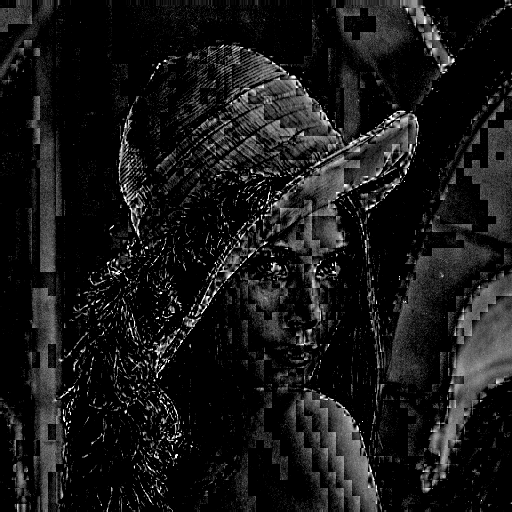
\includegraphics[width=5cm]{lena_q5_diff.png} \\
   \hline
   q = 20 & 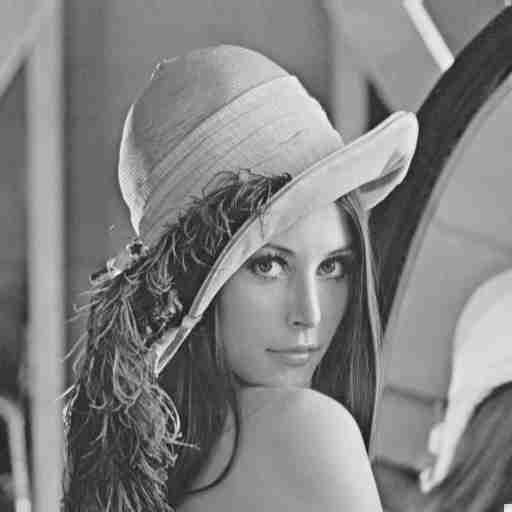
\includegraphics[width=5cm]{lena_q20.png} & 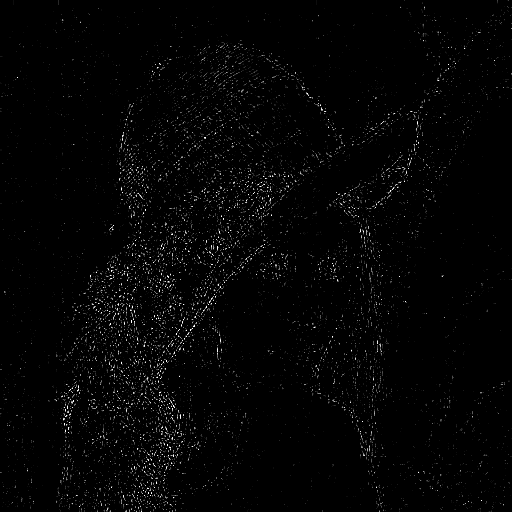
\includegraphics[width=5cm]{lena_q20_diff.png} \\
   \hline
   q = 50 & 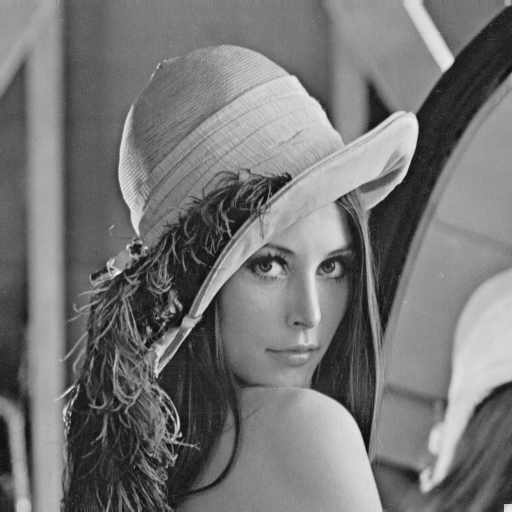
\includegraphics[width=5cm]{lena_q50.png} & 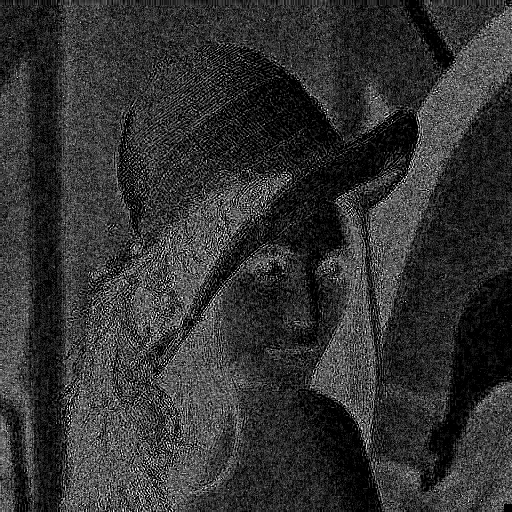
\includegraphics[width=5cm]{lena_q50_diff.png} \\
   \hline
   q = 75 & 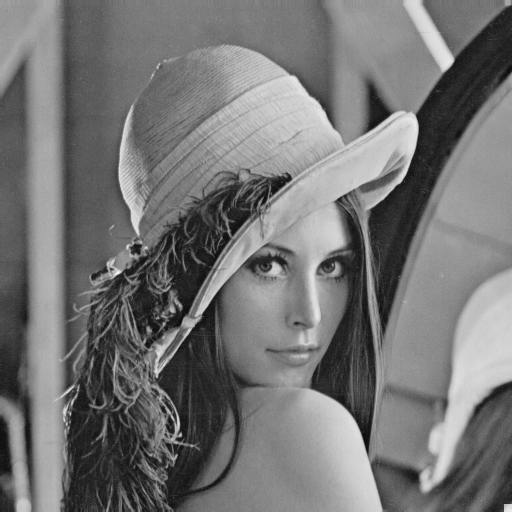
\includegraphics[width=5cm]{lena_q75.png} & 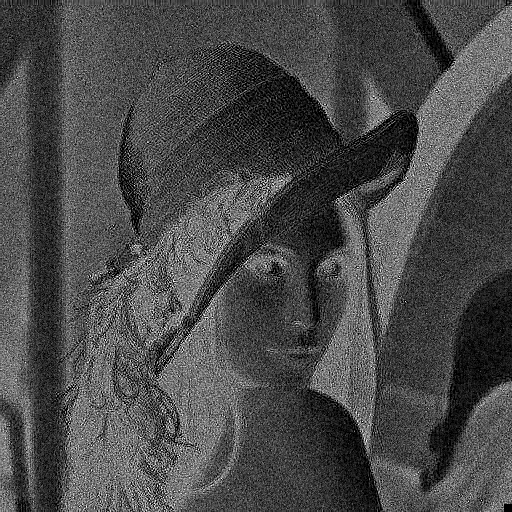
\includegraphics[width=5cm]{lena_q75_diff.png} \\
   \hline
  \end{tabular}

  
  %TODO tableau de résultat
  
  
\end{document}  